%-------------------------
% Resume in Latex
% Author : Sourabh Bajaj
% License : MIT
%------------------------

\documentclass[letterpaper,11pt]{article}

\usepackage{latexsym}
\usepackage[empty]{fullpage}
\usepackage{titlesec}
\usepackage{marvosym}
\usepackage[usenames,dvipsnames]{color}
\usepackage{verbatim}
\usepackage{enumitem}
\usepackage[pdftex]{hyperref}
\usepackage{fancyhdr}
\usepackage{zh_CN-Adobefonts_external}
\usepackage{graphicx}
\usepackage{multirow}


\pagestyle{fancy}
\fancyhf{} % clear all header and footer fields
\fancyfoot{}
\renewcommand{\headrulewidth}{0pt}
\renewcommand{\footrulewidth}{0pt}

% Adjust margins
\addtolength{\oddsidemargin}{-0.375in}
\addtolength{\evensidemargin}{-0.375in}
\addtolength{\textwidth}{1in}
\addtolength{\topmargin}{-.5in}
\addtolength{\textheight}{1.0in}

\urlstyle{same}

\raggedbottom
\raggedright
\setlength{\tabcolsep}{0in}

% Sections formatting
\titleformat{\section}{
  \vspace{-4pt}\scshape\raggedright\large
}{}{0em}{}[\color{black}\titlerule \vspace{-5pt}]

%-------------------------
% Custom commands
\newcommand{\resumeItem}[2]{
  \item\small{
    \textbf{#1}{: #2 \vspace{-2pt}}
  }
}

\newcommand{\resumeSubheading}[4]{
  \vspace{-1pt}\item
    \begin{tabular*}{0.97\textwidth}{l@{\extracolsep{\fill}}r}
      \textbf{#1} & #2 \\
      \textit{\small#3} & \textit{\small #4} \\
    \end{tabular*}\vspace{-5pt}
}

\newcommand{\resumeSubItem}[2]{\resumeItem{#1}{#2}\vspace{-4pt}}

\renewcommand{\labelitemii}{$\circ$}

\newcommand{\resumeSubHeadingListStart}{\begin{itemize}[leftmargin=*]}
\newcommand{\resumeSubHeadingListEnd}{\end{itemize}}
\newcommand{\resumeItemListStart}{\begin{itemize}}
\newcommand{\resumeItemListEnd}{\end{itemize}\vspace{-5pt}}

%-------------------------------------------
%%%%%%  CV STARTS HERE  %%%%%%%%%%%%%%%%%%%%%%%%%%%%

\begin{document}

%----------HEADING-----------------
\begin{tabular*}{0.8\textwidth}{l@{\extracolsep{\fill}}r}
    & \multirow{3}{4em}{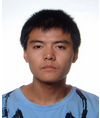
\includegraphics[height=3cm]{huizhu.png}} \\
    & \\
    Huizhu Zhao & \\
    Email : zhaohuizhu@ruc.edu.cn & \\
    Mobile : +86-180-0109-0187  & \\
    Blog : \href{https://huizhuzhao.github.io/}{https://huizhuzhao.github.io} & \\
    \textbf{Job intension} : \textbf{Machine learning (NLP or CV)} &
\end{tabular*}


%-----------EDUCATION-----------------
\section{Education}
\begin{itemize}
\item \textbf{Renmin University of China}  \qquad Beijing, China \\
    Master of theoretical physics \qquad \qquad Sep 2012 -- July 2015 \\
    Awarded "National Postgraduate Scholarship", "Outstanding Graduates in Beijing City"

\item \textbf{Hebei University of Technology} \qquad Tianjin, China \\
    Bachelor of Engineering Management \qquad Sep. 2008 -- July. 2012 \\
    Awarded "First Prize of Tianjin College Students Math Contest", \\
    "Second Prize of China Undergraduate Mathematics Contest in Modeling in Hebei Division", \\
    "Second Prize of Tianjin College Students Physics Contest"


\end{itemize}

\section{Research works}
\begin{itemize}
\item Deviation from the Maxwell-Cattaneo law: the role of the asymmetric interactions \\
Huizhu Zhao, Lei Wang \href{https://journals.aps.org/pre/abstract/10.1103/PhysRevE.92.042136}{Phys.Rev.E 92, 042136}
\item Heat-current correlation loss induced by finite-size effects in a one-dimensional nonlinear lattice \\
Lei Wang, Lubo Xu, Huizhu Zhao, \href{https://journals.aps.org/pre/abstract/10.1103/PhysRevE.91.012110}{Phys. Rev. E 91, 012110}
\end{itemize}

\section{Experience}
\begin{itemize}
\item Xtalpi \qquad  Algorithm Engineer \qquad April 2016 -- present \\
    In charge of the development of machine learning algorithms for molecular 
    phsical/chemical properties prediction. Including 
    \begin{itemize}
        \item the vectorization of molecular graph based on their 2D/3D topological and chemical 
            information; 
        \item building multitask neural model for drug/target activities prediction
        \item the vectorization of molecule-protein complexes for binding affinity prediction; 
        \item writing the toolkits for molecular info extraction from their files/strings 
            through API of \href{http://www.rdkit.org}{rdkit} and \href{http://openbabel.org/docs/current/index.html}{openbabel}; 
        \item collecting molecular/drug datasets (with python) from public chemical databases for training machine learning models;
    \end{itemize}
%\item XingTu Tech. \qquad Data Analyst \qquad \qquad Sep 2015 -- Nov 2015 \\
%    Participated in the data collection works extracted from several popular e-commence webs with python language.
\end{itemize}


 

\section{Projects}
\begin{itemize}


\item Convolutional Networks on Graphs for Learning Molecular Fingerprints (\href{https://arxiv.org/pdf/1509.09292.pdf}{paper}) \\
    This model implements convolutional nets which can take molecular graph of 
    arbitrary size as input, and the learned weights will be used to generate 
        molecular fingerprints for classification/regression tasks.  (written in lasagne and tensorflow)
\item Neural Message Passing for Quantum Chemistry (\href{https://arxiv.org/abs/1704.01212}{paper}) \\
    This message passing algorithm reformulates existing neural network models into a single common framework (MPNN) 
    to compute the mapping function of the input molecular graph into an efficient features for molecular chemical properties
    prediction with state of art accuracy.
\item Massively Multitask Networks for Drug Discovery (\href{https://arxiv.org/abs/1502.02072}{paper}) \\
    This work applied multitask neural architectures which achieves significant approvements over baseline ML models on drug discovery.

\item Quantum-chemical insights from deep tensor neural networks (\href{https://www.nature.com/articles/ncomms13890}{paper}) \\
    An neural network model for prediction of quantum-mechanical observables of molecular systems
\item Global AI Hackathon $\cdot$ Beijing (factial expression recgonition) \\
    This is a two days' hackathon, and our team (mainly 3 members) won the first place with VGG net which reaches a
        recognition accuracy of 57\%. \href{https://github.com/huizhuzhao/Hackthon/tree/master/xlyte}{code}

\end{itemize}


\section{Skills}
\begin{itemize}
    \item language: python, C (have MPI parallel computing experience during college), familiar with Linux os
    \item ML frameworks: tensorflow, keras (most frequently use), theano, lasagne
    \item English: TOEFL--93, GRE--322+3.0
\end{itemize}

\section{my words}
I am ethusiastic about developing advanced machine learning algorithms to harness the explosion of 
digital data and computational power to create more intelligent computer systems.

%-------------------------------------------
\end{document}
